\documentclass[a4paper]{article}
\usepackage{ucs}
\usepackage[T2A]{fontenc}
\usepackage[utf8]{inputenc}
\usepackage[english,bulgarian]{babel}
\usepackage{graphicx}
\usepackage{url}
\usepackage{textcomp}
\usepackage{amsmath}
\usepackage{amsfonts}
\usepackage{amssymb}
\usepackage{tabularx}
\usepackage{array}
\usepackage[margin=1.5in]{geometry}
\usepackage[unicode]{hyperref}

\usepackage{fancyhdr}
\setlength{\headheight}{15pt}
 
\pagestyle{fancyplain}

\usepackage{listings}

\addto\captionsbulgarian{%
  \renewcommand{\contentsname}%
    {Содржина}%
  \renewcommand{\tablename}%
    {Табела}%
  \renewcommand{\figurename}%
    {Слика}%
  \renewcommand{\bibname}%
    {Библиографија}%
  \renewcommand{\listfigurename}%
    {Листа на слики}%
  \renewcommand{\listtablename}%
    {Листа на табели}%
}

\rhead{\textsc{Структурно програмирање}}
\chead{}
\lhead{Домашна задача 1}
\lfoot{}
\cfoot{\thepage}
\rfoot{}
\usepackage{fancyvrb}
\usepackage{xcolor}
\usepackage{textcomp}

\begin{document}


\section{Што е Code?}

Code е веб систем за автоматско компајлирање, извршување и оценување задачи
од програмирање. На овој веб систем ќе  се работат лабораториските вежби и ќе се
изведуваат сите колоквиуми и испити по предметот Структурно програмирање.

\begin{figure}[htbp]
\centering
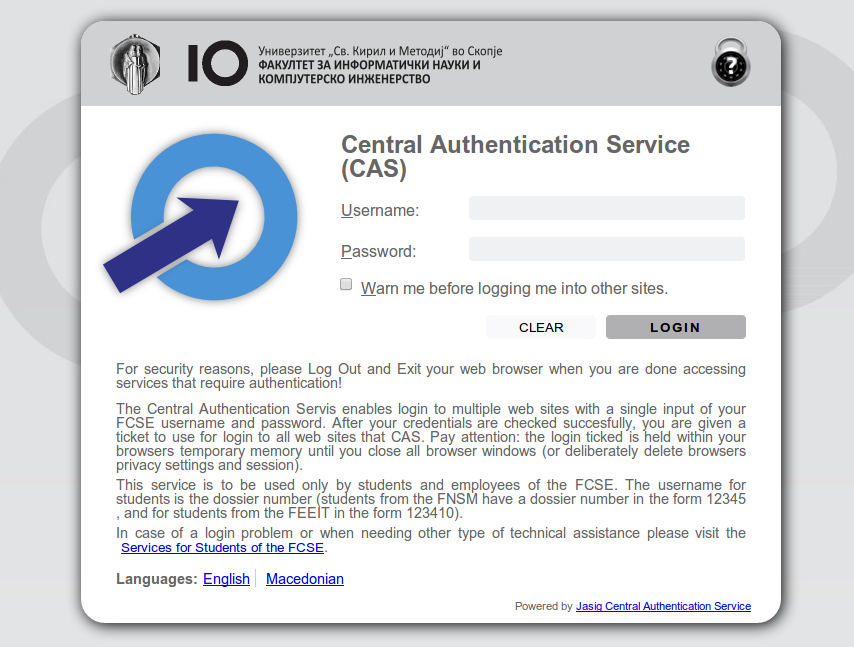
\includegraphics[width=0.7\textwidth]{images/code/cas}
\caption{CAS системот за најавување}
\end{figure}

\begin{figure}[htbp]
\centering

\includegraphics[width=\textwidth]{images/code/main}
\caption{Почетен изглед на системот откако ќе се најавите}
\end{figure}

\subsection{Адреса и најавување}

На системот може да пристапите преку било кој веб прелистувач (препорачани и
тестирани Google Chrome и Mozilla Firefox) преку следната веб локација:

\begin{verbatim}
http://code.finki.ukim.mk/
\end{verbatim}

Најавувањето се прави преку сервисот за централна автентикација (Central
Authentication Service (CAS)) со вашето корисничко име (индекс) и лозинка.

\subsection{Избор на предмет}

Откако ќе се најавите добивате листа со линкови до предметите кои ги слушате и
го користат системот за лабораториски вежби. Го избирате соодветниот предмет со
клик на линкот (Структурно програмирање).

\subsection{Листа со лабораториски вежби и задачи}

\begin{figure}[htbp]
\centering
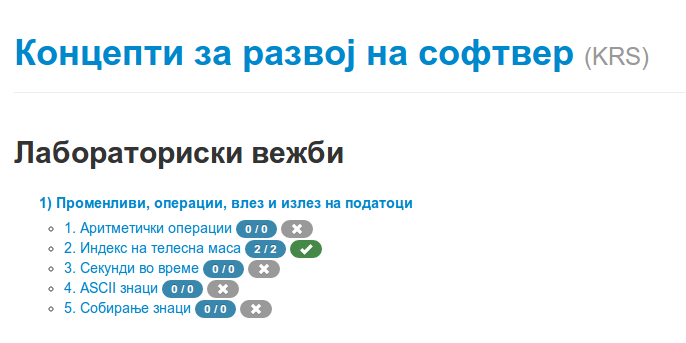
\includegraphics[scale=.5]{images/code/krs}
\caption{Листа со лабораториски вежби и задачи}
\end{figure}

На овој поглед ви се прикажани линкови до сите активни лабораториски вежби и
нивните задачи. Пристапувањето до соодветната задача е со клик на линкот. До
секоја задача има број (пр. 1/4) и икона кои го прикажуваат бројот на успешни
обиди од бројот на вкупно обиди и тоа дали има барем еден успешен обид за
рашавање на задачата.

\begin{figure}[htbp]
\centering
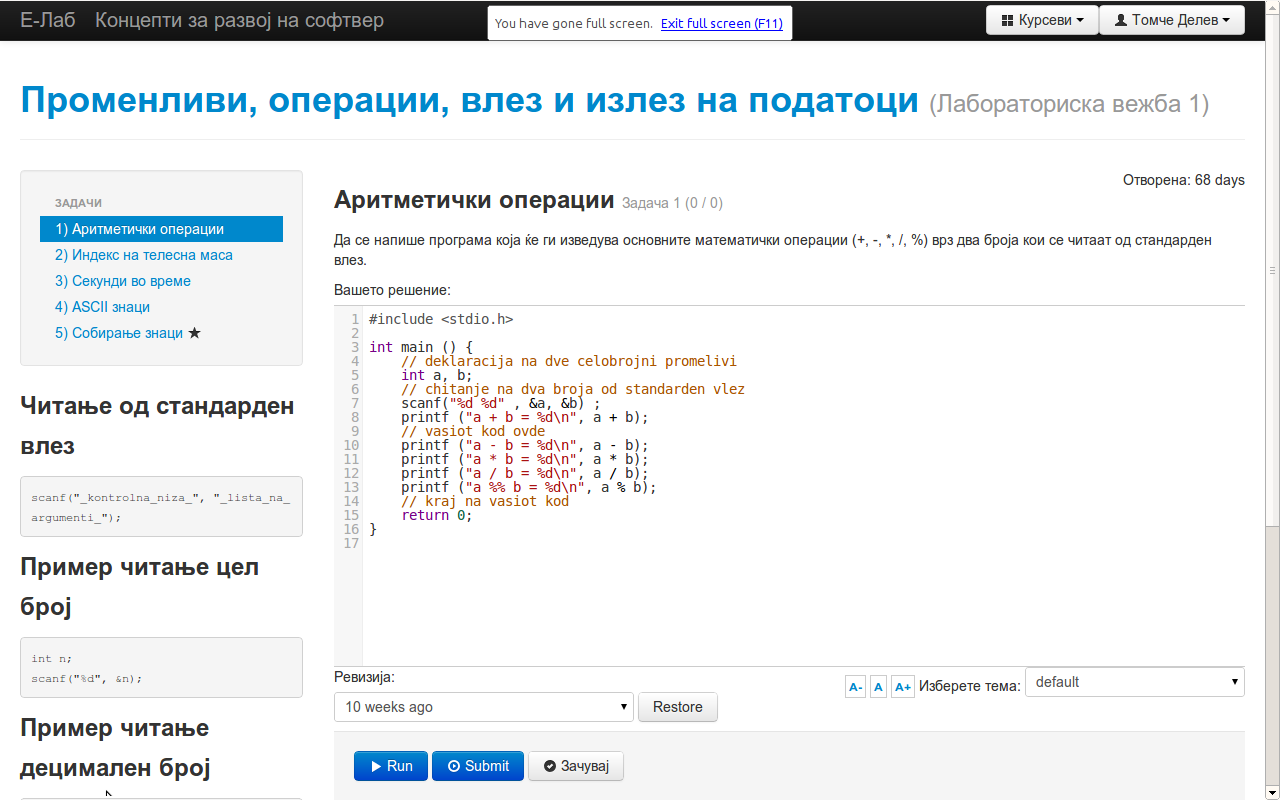
\includegraphics[width=\textwidth]{images/code/screen}
\label{fig:screen}
\caption{Поглед за решавање на задача}
\end{figure}

\subsection{Опис на погледот за решавање на задача}

Откако ќе се кликне на линкот до одредена задача се преминува на погледот за
решавање на задачата (слика \ref{fig:screen}). Во овој поглед се работи на
решавање на дадената задача и се тестира и поднесува решението.

Погледот се состои од името и текстот на задачата (слика \ref{fig:text}),
текстуален едитор за внесување на кодот на решението на задачата (слика
\ref{fig:editor}), панел со можни акции врз кодот на вашето решение (слика
\ref{fig:actions}), приказ на излезот од извршувањето на програмата (слика
\ref{fig:output}), панел со помош за дадената задача (слика \ref{fig:help}) и
листа за пристап до останатите задачи од дадената лабораториска вежба
(\ref{fig:problems}).

\begin{figure}[htbp]
\centering

\includegraphics[scale=.4]{images/code/text}
\caption{Име и текст на задачата}
\label{fig:text}
\end{figure}

\begin{figure}[htbp]
\centering
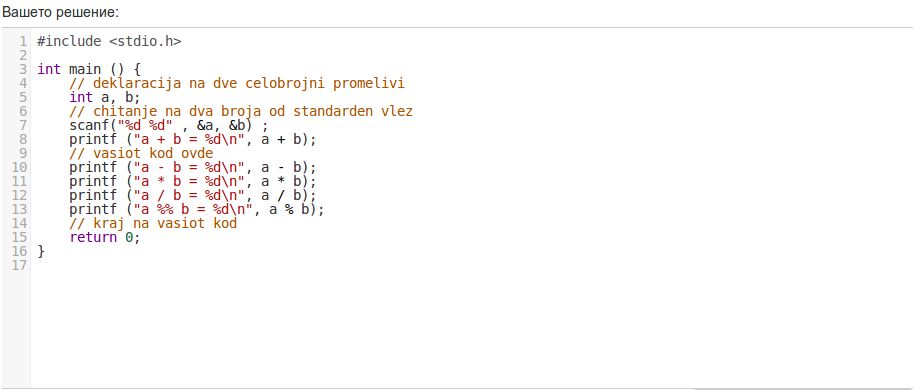
\includegraphics[scale=.4]{images/code/editor}
\caption{Текстуален едитор за внесување на кодот на решението}
\label{fig:editor}
\end{figure}

\begin{figure}[htbp]
\centering

\includegraphics[scale=.4]{images/code/actions}
\caption{Панел со можни акции со кодот на вашето решение}
\label{fig:actions}
\end{figure}

\begin{figure}[htbp]
\centering
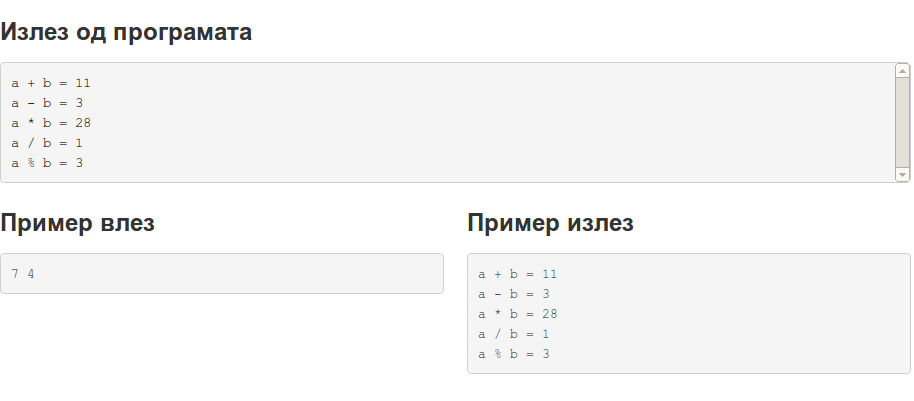
\includegraphics[scale=.5]{images/code/output}
\caption{Приказ на излезот од извршувањето на програмата}
\label{fig:output}
\end{figure}

\begin{figure}[htbp]
\centering
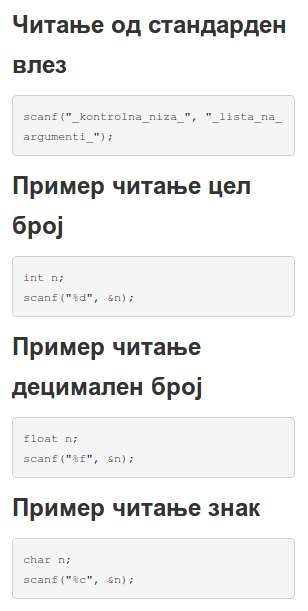
\includegraphics[scale=.5]{images/code/help}
\caption{Панел со помош за дадената задача}
\label{fig:help}
\end{figure}

\begin{figure}[htbp]
\centering
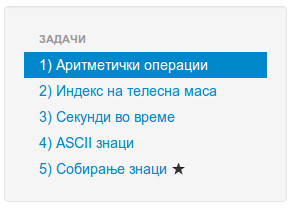
\includegraphics[scale=.5]{images/code/problems}
\caption{Листа за пристап до сите задачи од дадената лабораториска вежба}
\label{fig:problems}
\end{figure}

\subsection{Како се извршува и поднесува решение}

Откако детално ќе го прочитате текстот на задачата, ќе ги разгледате пример
влезот и излезот на дадената задача, започнувате со размислување и работа на
решението на задачата. Кодот од решението го внесувате во текстуалниот едитор
(слика \ref{fig:editor}) и откако ќе внесете код кој сакате да го тестирате на
дадениот пример влез, со клик на копчето \texttt{Run} од панелот за акции
(слика \ref{fig:actions}), вашата програма ќе се \textbf{компајлира} и
\textbf{изврши} со читање на пример влезот од стандарден влез и печатење на
излезот од вашето решение во панелот за приказ на резултатот од извршувањето
(слика \ref{fig:output}).

Ако вашиот код содржи грешки и не може да се искомпајлира, системот во панелот
за приказ на резултатот од извршувањето на програмата ќе ви ги прикаже
соодветните грешки во црвена боја (слика \ref{fig:errors}).

\begin{figure}[htbp]
\centering
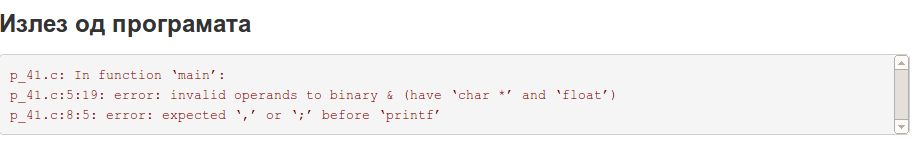
\includegraphics[scale=.4]{images/code/errors}
\caption{Приказ на грешки од процесот на компајлирање}
\label{fig:errors}
\end{figure}

Откако ќе ги исправите евентуалните грешки при компајлирање на програмата и
вашата програма се извршува точно на дадениот пример влез, може да го поднесете
ова решение да се тестира и на останатите тест примери со клик на копчето
\texttt{Submit}.

По извршување на оваа акција системот ќе ја изврши програмата со влез од сите
тест примери, при што ќе го спореди излезот со соодветниот излез од тест
примерот. Резултатот од ова тестирање се прикажува на приказот на слика
\ref{fig:results}. Ако излезот на сите тест примери од вашата програма е ист со
излезот на дадените тест примери, тогаш вашето решение е точно и може да
преминете на решавање на друга задача.

\begin{figure}[htbp]
\centering
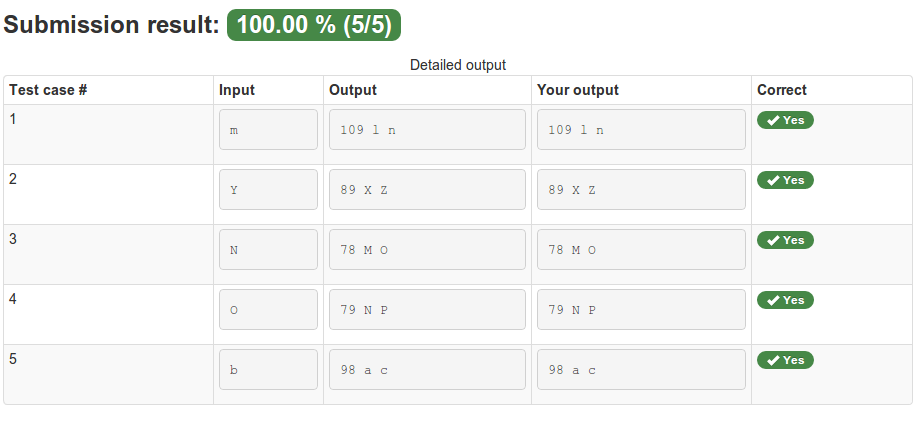
\includegraphics[scale=.4]{images/code/results}
\caption{Приказ на резултатите од поднесувањето на решението}
\label{fig:results}
\end{figure}

\section{Вежба}

Во вашата прва вежба, откако ќе се запознаете со системот треба да се обидете
самостојно да ги решите дадените 5 задачи и да ги поднесете вашите решенија
(\texttt{Submit}).

\section{Прашања}

Ако имате прашања, нејаснотии или желби за системот, пишете на
\begin{verbatim}
tdelev@finki.ukim.mk
\end{verbatim}

Ви посакуваме успешна работа и многу точни решенија на задачите од
лабораториските вежби по предметот Концепти за развој на софтвер.

\end{document}
